\chapter{Chemische Reaktionsnetzwerke}

\begin{definition}[Atom map]
    Seien $ S_1 = (V_1, E_1)$, $ S_2 = (V_2, E_2) $ zwei Stoff-Graphen und $ P = (V, E) $ der Produkt Graph einer chemischen Reaktion.
    Dann ex. eine \textit{atom map} $ a : V_1 \cup V_2 \rightarrow V $, die bijektiv ist (vgl. Abb. \ref{fig:atom-map}).
\end{definition}

\begin{figure}
    \centering
    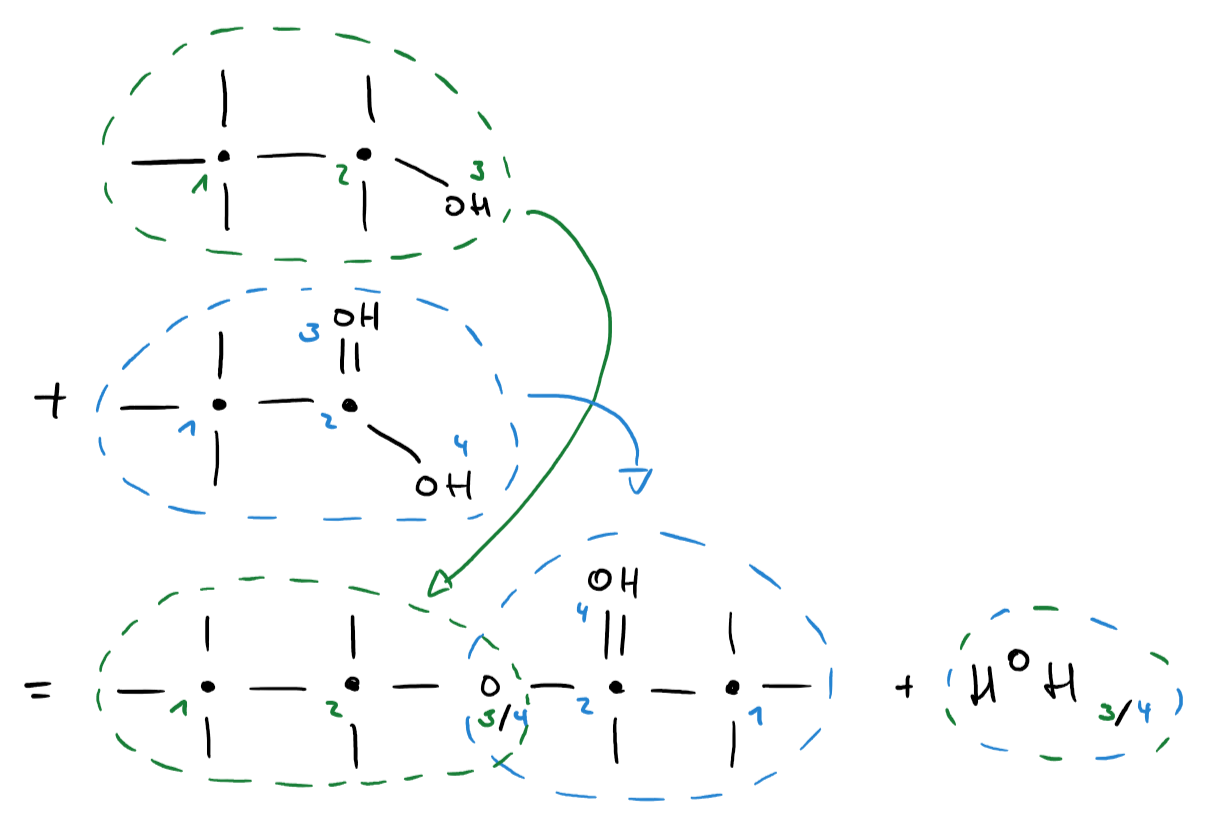
\includegraphics[width=0.75\textwidth]{figures/chem.png}
    \caption{Beispiel für atom map}
    \label{fig:atom-map}
\end{figure}

\begin{remark}
    Um atom maps zu berechnen, kann das maximum common subgraph Problem (MCS) gelöst werden.
    Das Berechnen von Atom maps ist eine Standardanwendung von Subgraph-Isomorphie Algorithmen.
    Dies funktioniert gut, wenn die Reaktion nur kleine Änderungen an den Graphen vorgenommen hat.
    Schlecht funktioniert die Anwendung des MCS, wenn sehr ähnliche Graphen miteinander reagieren.
\end{remark}

\begin{definition}[Monomorphismus]
    Seien $ G = (V_G, E_G) $ und $ H = (V_H, E_H)  $ zwei Graphen.
    Eine Funktion $ m : V_G \rightarrow V_H $ ist ein Monomorphismus, falls:
    \begin{enumerate}
        \item $ m $ injektiv ist und
        \item für $ v_1, v_2 \in V_G $ gilt, dass wenn $ \{ v_1, v_2 \} \in E_G $, dann $ \{ m(v_1), m(v_2) \} \in E_H $.
    \end{enumerate}

    Im chemischen Kontext wird zusätzlich gefordert, dass $ m $ auch surjektiv, also insgesamt bijektiv sein muss (vgl. Abb. \ref{fig:monomorphism}).
\end{definition}

\begin{figure}
    \centering
    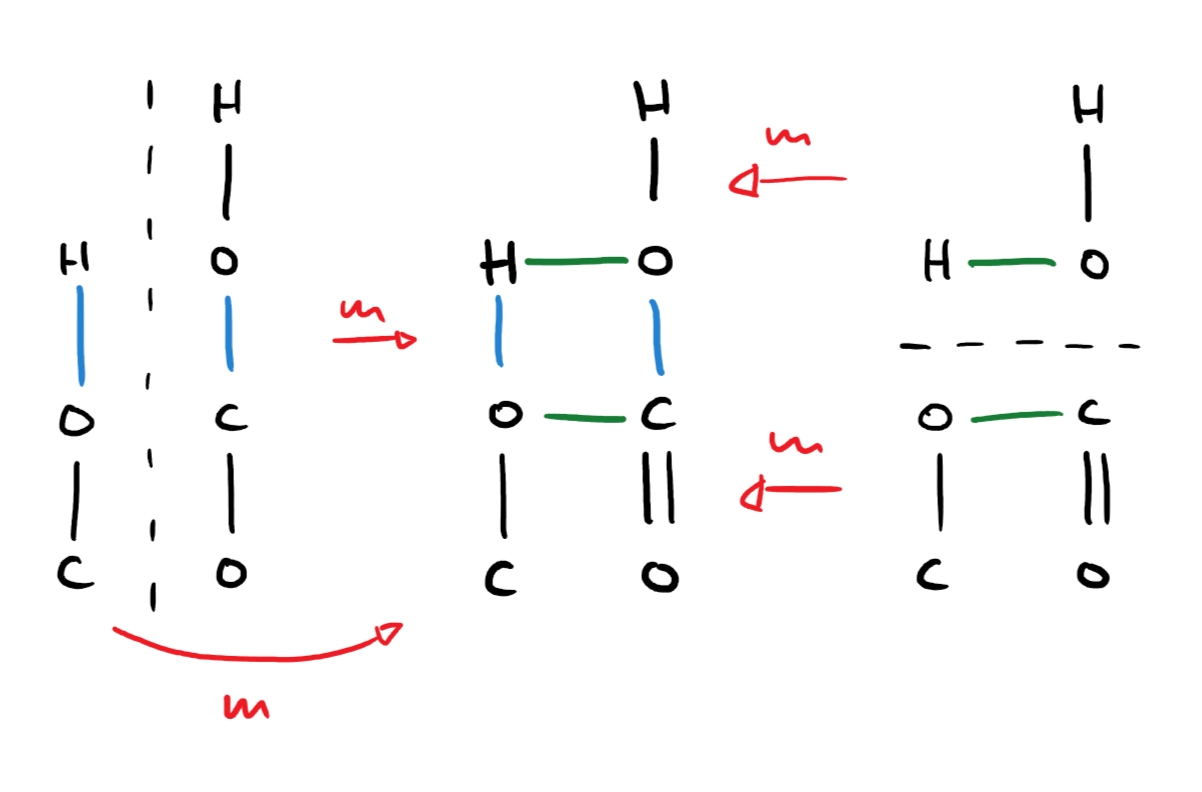
\includegraphics[width=0.75\textwidth]{figures/monomorphism.png}
    \caption{Monorphismus Beispiel}
    \label{fig:monomorphism}
\end{figure}

\begin{remark}[DPO-Modell]
    Über Monomorphismen können Graph-Ersetzung-Regeln definiert werden.
    Dies geschieht bspw. im \textbf{D}ouble-\textbf{P}ush-\textbf{O}ut Modell (DPO).
    Eine Graph Regel ist dort ein Tripel $ (L, K, R) $ mit zwei Monomorphismen $ m_l : K \to L $ und $ m_r : K \to R $.
    Knapp zusammengefasst:
    \begin{itemize}
        \item $ K $ ist eine Vorbedingung, die man in einem Eingabegraphen ``finden'' können muss, um die Regel anzuwenden.
        \item $ L $ ist der Teil des Eingabegraphen, der gelöscht wird.
        \item $ R $ ist der Teil des Eingabegraphen, der hinzugefügt wird.
    \end{itemize}

    Eine Ersetzung verläuft dann in diesen Schritten (vgl. Abb. \ref{fig:dpo}; Pfeile veranschaulichen Monomorphismen):
    \begin{enumerate}
        \item Finde einen ``glue''-Graphen $ D $, der zusammen mit $ L $ wieder $ G $ ergibt und zu dem ein Monomorphismus von $ K $ aus existiert.
        Des Weiteren muss ein Monomorphismus von $ D $ nach $ G $ existieren.
        \item Verwende $ D $, um den Ergebnisgraphen $ H $ zu erzeugen.
        Dieser ergibt sich aus der ``Summe'' von $ R $ und $ D $.
        Wieder existiert ein Monomorphismus von je $ R $ und $ D $ nach $ H $.
    \end{enumerate}

    \begin{figure}
        \centering
        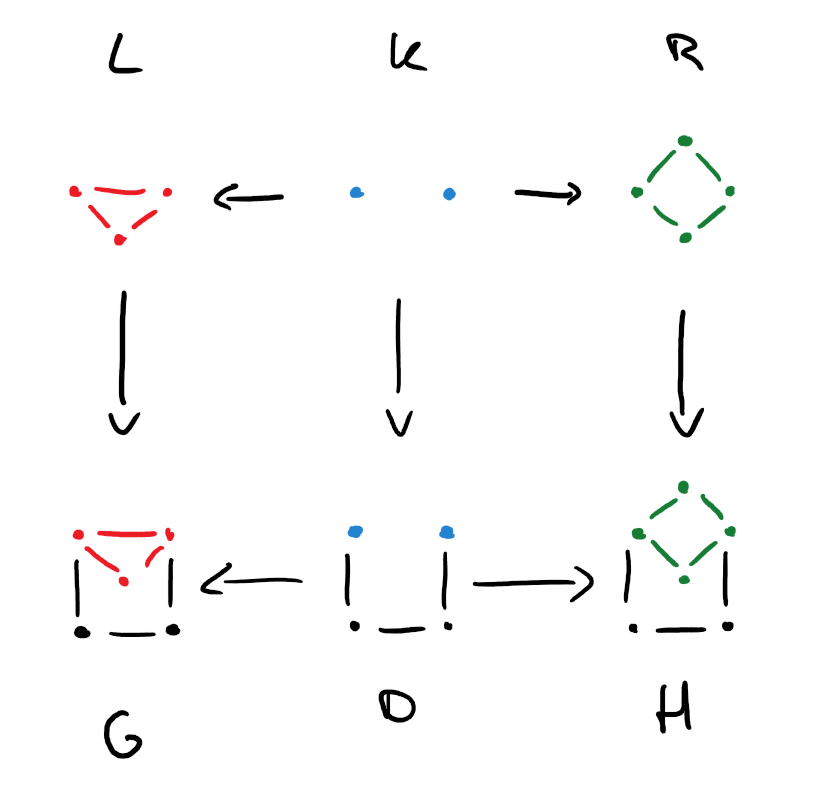
\includegraphics[width=0.75\textwidth]{figures/dpo.png}
        \caption{DPO}
        \label{fig:dpo}
    \end{figure}
\end{remark}
